\documentclass{scrartcl}
\usepackage[T1]{fontenc}
\usepackage{ntheorem}

\usepackage{amsmath}
\DeclareMathOperator{\Res}{Res}
\usepackage{mathpazo}
\usepackage{graphicx}
\newcommand{\R}{\mathbb{R}}

\newcommand*{\vertbar}{\rule[-1ex]{0.5pt}{2.5ex}}
\newcommand*{\horzbar}{\rule[.5ex]{2.5ex}{0.5pt}}

\begin{document}
\title{Linear Algebra and Learning from Data}
\subtitle{Chapter 1}
\author{Selected solutions by Benjamin Basseri}
\date{}
\maketitle

\begin{enumerate}
	\item Give an example where a combination of three nonzero vectors in $\R^4$ is the zero vector. Then write your example in the form $Ax = 0$. What are the shapes of $A, x$ and 0?

We can choose two vectors then make the third vector a linear combination of the first two:
$$\mathbf{a} + \mathbf{b} + (\lambda_1 \mathbf{a} + \lambda_2 \mathbf{b})$$

In this case we may choose:
$$a = \begin{bmatrix}
	1 \\ 0 \\ 0 \\ 0
\end{bmatrix}, 
b = \begin{bmatrix}
	0 \\ 1 \\ 0 \\ 0
\end{bmatrix},
c = \begin{bmatrix}
	1 \\ 1\\ 0 \\ 0
\end{bmatrix}$$

Then $a + b - c = 0$. This linear combination of $a, b, c$ can be expressed in matrix form as:
$$[a \ b \ c] \begin{bmatrix}
	1 \\ 1 \\ -1
\end{bmatrix} = 
\begin{bmatrix}
	1 & 0 & 1 \\
	0 & 1 & 1 \\
	0 & 0 & 0 \\ 
	0 & 0 & 0 \\
\end{bmatrix}
\begin{bmatrix}
	1 \\ 1 \\ -1
\end{bmatrix} = \mathbf{0}$$

where $A$ is $4 \times 3$, $x$ is $3 \times 1$, and 0 is $3\times 1$.

\item Suppose a combination of the columns of $A$ equals a different combination of those columns. Write that as $Ax = Ay$. Find two combinations of the columns of $A$ that equal the zero vector (in matrix language, find two solutions to $Az = 0$).

$$Ax = Ay \implies Ax - Ay = 0 \implies A(x-y) = 0 \implies x-y \in \ker A$$

This also implies $y-x$ is in the null space of $A$ since we could subtract $Ax$ from both sides in the first step just as well.

\item The vectors $\mathbf{a}_1, \mathbf{a}_2, \ldots, \mathbf{a}_n$ are in $m$-dimensional space $\R^m$, and a combination $c_1\mathbf{a}_1 + \ldots + c_n \mathbf{a}_n$ is the zero vector. That statement is at the vector level.
\begin{enumerate}
	\item Write that statement at the matrix level. Use the matrix $A$ with the $\mathbf{a}$'s in its columns and use the column vector $\mathbf{c} = (c_1, \ldots, c_n)$.

One of Strang's pictures of matrix multiplication describes $A\mathbf{c}$ as a linear combination of the columns of $A$, with the combination given by the components of $\mathbf{c}$. Thus
\[
A\mathbf{c} = 
\left[
  \begin{array}{cccc}
    \vertbar & \vertbar &        & \vertbar \\
    \mathbf{a}_{1}    & \mathbf{a}_{2}    & \ldots & \mathbf{a}_{n}    \\
    \vertbar & \vertbar &        & \vertbar 
  \end{array}
\right]\begin{bmatrix}
	c_1 \\ \vdots \\ c_n
\end{bmatrix} = 0
\]
$$\iff c_1 \mathbf{a}_1 + \ldots c_n \mathbf{a}_n = 0$$


	\item Write that statement at the scalar level. Use subscripts and sigma notation to add up numbers. The column vector $\mathbf{a}_j$ has components $a_{1j}, a_{2j}, \ldots, a_{mj}$.

From the matrix picture we can write out in summation for the $j$th component of $A\mathbf{c}$:
$$(A\mathbf{c})_j = \sum_{i=0}^m c_i a_{ji} = 0$$
$$\text{altogether: } A\mathbf{c} = \sum_{j=1}^n \sum_{i=1}^m c_i a_{ij}\mathbf{e}_j = \mathbf{0}$$
\end{enumerate}

\item Suppose $A$ is the 3 by 3 matrix of all ones. Find two independent vectors $x$ and $y$ that solve $Ax = 0$ and $Ay = 0$. Write that first equation $Ax = 0$ (with numbers) as a combination of the columns of $A$. Why don't I ask fo ra third independent vector with $Az = 0$?

We can choose $x = (1, -1, 0), y = (0, 1, -1)$. These are independent since clearly there is no scalar $\lambda$ such that $\lambda x = y$: the scalar $\lambda $ would have to map $x_1 \mapsto 0$ which implies $\lambda = 0$, but then $x_2 \mapsto 1$ which implies $\lambda \neq 0$. 

Let $\mathbf{1}$ be the vector of 1's, which in this case is each column of $A$. Then
$$Ax = \sum_{i=1}^3 x_i \mathbf{1} = x_1 \mathbf{1} + x_2 \mathbf{1} + x_3\mathbf{1} = 1\cdot \mathbf{1} - 1\cdot\mathbf{1} + 0 = 0$$

There is no 3rd independent vector in the null space of $A$. This follows from rank-nullity: $A$ has a rank of 1, its column space is the subspace spanned by $\mathbf{1}$ (a line). Since we're in $\R^3$, that means $N(A)$ has dimension 2.

\item The linear combinations of $v =(1, 1, 0)$ and $w = (0, 1, 1)$ fill a plane in $\R^3$.
\begin{enumerate}
	\item Find a vector $z$ that is perpendicular to $Wv$ and $w$. 

Such a vector $z$ must have a 0 dot product with $v$ and $w$. By inspection we see that if $z = (1, -1, 1)$ then the dot product with either $v$ or $w$ will get a 1 from the first or third component and a -1 from the second:

$$z \cdot v = \begin{bmatrix}
	1 \\ -1 \\ 1
\end{bmatrix}\cdot
\begin{bmatrix}
	1 \\ 1 \\0
\end{bmatrix} = 0$$
$$z \cdot w = \begin{bmatrix}
	1 \\ -1 \\ 1
\end{bmatrix}\cdot
\begin{bmatrix}
	0 \\ 1 \\ 1
\end{bmatrix} = 0$$

\item Find a vector $u$ that is not on the plane. Check that $u^\top z \neq 0$


	Of course $z$ is not in the plane and since $z \neq 0$, we have $z^\top z \neq 0$.
\end{enumerate}

\item If three corners of a parallelogram are (1,1), (4,2), and (1,3), what are all three of the possible fourth corners? Draw two of them.

By the parallelogram rule of vector addition, we can take the vector represented by a point $x$ and add the other two points' \emph{differences} to $x$ to get the fourth point of the parallelogram. Starting at $(1,1)$, we have differences to $(1, 3)$ and $(4,2)$ as follows:
$$(1,3) - (1,1) = (0, 2), \quad (4,2) - (1,1) = (3,1)$$

so a point that makes a parallelogram would be (1,1) + (0, 2) + (3,1) = (4, 4).
\begin{center}
	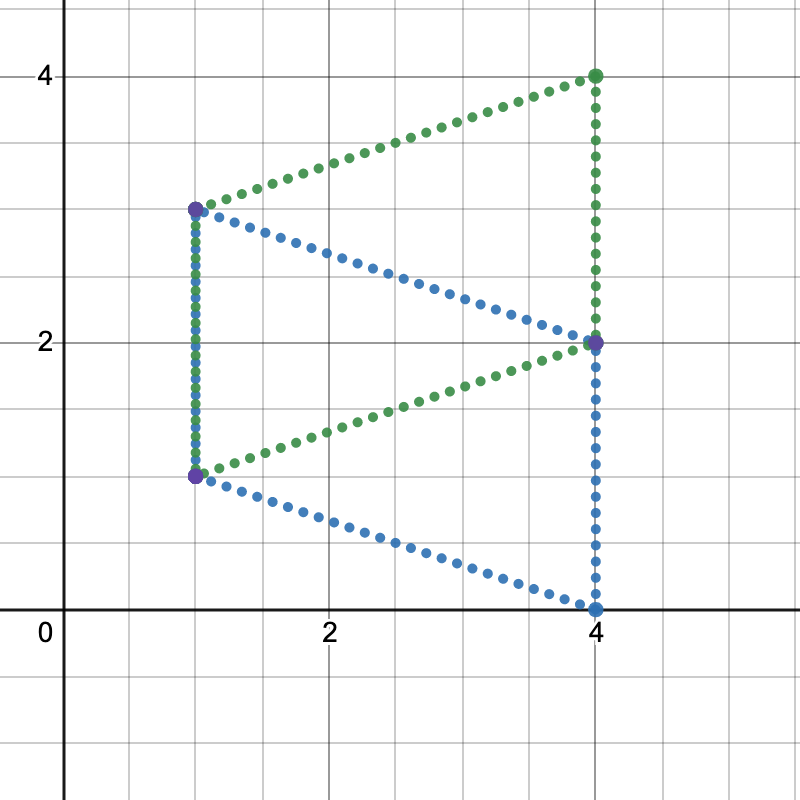
\includegraphics[width=0.5\textwidth]{imgs/1.1.6.png}
\end{center}

\item Describe the column space of $A = [v \ w \ v+2w]$. Describe the nullspace of $A$: all vectors $x = (x_1, x_2, x_3)$ that solve $Ax = 0$. Add the ``dimensions'' of that plane (the column space of $A$ and that line (the nullspace of $A$).

Let $C(A)$ denote the column space of $A$. Since the 3rd column is a linear combination of the first 2, $C(A) = C([v, w]) = \text{span}\{v, w\}$. Assuming $w \neq \lambda v$ the null space $N(A) = \{(1, 2, -1)\}$, since for any $x \in N(A) = \lambda(1, 2, -1)$ for some $\lambda$, then 
$$Ax = \lambda A(1,2,-1) = v + 2w - (v + 2w) = 0$$

$A$ spans a 2-dimensional plane and the nullspace is 1-dimensional, in keeping with rank-nullity.

\item $A = CR$ is a representation of the columns of $A$ in the basis formed by the columns of $C$ with coefficients in $R$. If $A_{ij} = j^2$ is 3 by 3, write down $A$ and $C$ and $R$. 

Given the recipe $A_{ij} = j^2$ we have
$$A = \begin{bmatrix}
	1 & 4 & 9 \\	1 & 4 & 9 \\	1 & 4 & 9 \\
\end{bmatrix}$$

The columns of $A$ are linearly dependent, we may keep the first column for $C$ and then $R$ is the matrix necessary to make $CR = A$:
$$C = \begin{bmatrix}
	1 \\ 1 \\ 1
\end{bmatrix}, \quad R = \begin{bmatrix}
	1 & 4 & 9
\end{bmatrix}$$

\item Suppose the column space of an $m \times n$ matrix is all of $\R^3$. What can you say about $m$? What can you say about $n$? What can you say about the rank $r$?

Given the span of a matrix is $\R^3$ it must be $m = 3$ and $n \geq 3$. If $m$, the number of rows, was any less than 3 it would not be able to span $\R^3$ (we omit the possibility that $m > 3$ and it spans a 3-dimensional subspace isomorphic to $\R^3$). Likewise if the number of columns $n$ is less than 3 then the matrix could not have 3 linearly independent vectors, which are necessary to form a minimally spanning set of $\R^3$. Altogether this means the rank $r$ of the matrix is 3.

\item Find the matrices $C_1$ and $C_2$ containing independent columns of $A_1$ and $A_2$:

$$A_1 = \begin{bmatrix}
	1 & 3 & -2\\3 & 9 & -6\\2 & 6 & -4
\end{bmatrix}, \qquad A_2 = \begin{bmatrix}
	1 & 2 & 3 \\ 4 & 5 & 6 \\ 7 & 8 & 9
\end{bmatrix}$$

For $A_1$ we see its second and third columns are multiples of the first. So $C_1 = \begin{bmatrix}
	1 \\ 3 \\ 2
\end{bmatrix} $.

For $A_2 = \begin{bmatrix}
	\mathbf{a}_1 & \mathbf{a}_2 & \mathbf{a}_3
\end{bmatrix}$ we see the third column is a linear combination of the other two: $\mathbf{a}_3 = 2\mathbf{a}_2 - \mathbf{a}_1$. The first two columns are linearly independent which makes $C_2 = \begin{bmatrix}
	1 & 2 \\ 4 & 5 \\ 7 & 8
\end{bmatrix}$

\item Factor each of those matrices into $A = CR$. The matrix $R$ will contain the numbers that multiply the columns of $C$ to recover columns of $A$. 

Having identified which columns are linearly columns of which, we encode that information into $R$:
$$C_1 = \begin{bmatrix}
	1 \\ 3 \\ 2
\end{bmatrix}, \qquad R_1 = \begin{bmatrix}
		1 & 3 & -2
\end{bmatrix}$$
$$ C_2 = \begin{bmatrix}
	1 & 2 \\ 4 & 5 \\ 7 & 8
\end{bmatrix}, \qquad R_2 = \begin{bmatrix}
	1 & 0 & -1 \\ 0 & 1 & 2
\end{bmatrix}$$

\begin{align*}
	&\begin{bmatrix}
		1 & 0 & -1 \\ 0 & 1 & 2
	\end{bmatrix}\\
	\begin{bmatrix}
		1 & 2 \\ 4 & 5 \\ 7 & 8
	\end{bmatrix}& \begin{bmatrix}
		1 & 2 & 3 \\
		4 & 5 & 6\\
		7 & 8 & 9
	\end{bmatrix}
\end{align*}

\item Produce a basis for the column spaces of $A_1$ and $A_2$. What are the dimensions of those columns spaces -- the number of independent vectors? What are the ranks of $A_1$ and $A_2$? How many independent rows in $A_1$ and $A_2$?

By construction the columns of $C_1$ and $C_2$ form bases for $A_1$ and $A_2$ since they are sets of linearly independent vectors that span the column space of the matrix. So we may choose for bases $B_1$ and $B_2$:

$$B_1 = \left\{\begin{bmatrix}
	1 \\ 3 \\ 2
\end{bmatrix}\right\}, \qquad B_2 = \left\{\begin{bmatrix}1 \\ 4 \\ 7\end{bmatrix}, \begin{bmatrix}
	2 \\ 5 \\ 8
\end{bmatrix}\right\}$$

The dimension of each column space is the number of linearly independent vectors in each basis. Hence $\dim C(A_1) = 1, \dim C(A_2) = 2$. Equivalently, these are the ranks of matrices $A_1$ and $A_2$. Lastly, the rank of $A$ is equal to the rank of $A^\top$ for a square $A$, so the matrices have the same number of independent rows as they do columns.

\item Create a 4 by 4 matrix of rank 2. What shapes are $C$ and $R$? 

Before construction, we know the shape of $C$ will be $4 \times 2$. It must have 4 rows since it much match the original matrix. It will have 2 columns since we're constructing the original matrix to have 2 linearly independent columns.

Let us construct the matrix:
$$A = \begin{bmatrix}
	1 & 0 & 1 & -1 \\ 0 & 1 & 1 & -1 \\ 0 & 0 & 0 & 0 \\ 0 & 0 & 0 & 0 
\end{bmatrix}$$

The first two columns of $A$ are independent and the second two are linear combinations of the others. This gives $C$ and $R$:

\begin{align*}
	&\begin{bmatrix}
		1 & 0 & 1 & -1 \\ 0 & 1 & 1 & -1
	\end{bmatrix}\\
	\begin{bmatrix}
		1 & 0 \\ 0 & 1 \\ 0 & 0 \\ 0 & 0
	\end{bmatrix}&\begin{bmatrix}
	1 & 0 & 1 & -1 \\ 0 & 1 & 1 & -1 \\ 0 & 0 & 0 & 0 \\ 0 & 0 & 0 & 0 
\end{bmatrix}
\end{align*}

\item Suppose two matrices $A$ and $B$ have the same column space.
\begin{enumerate}
	\item Show that their row spaces can be different
\end{enumerate}

\end{document}